\chapter{RB fidelity optimization}
The calibration procedure described in Section \ref{sec:calibration} is typically time-consuming and demands significant experimental expertise, particularly when aiming for state-of-the-art performance. 
In the work presented in the previous chapter, the calibration process began from a pre-existing, even if suboptimal, configuration. 
The goal was to enhance the quality of single-qubit gates using the available \Qibocal protocols.

Even under these overall favorable initial conditions, the effort required to refine gate performance showed the limitations of manual calibration approaches. 
As quantum processors scale in both qubit count and architectural complexity, calibration becomes increasingly difficult. 
Frequent recalibrations are necessary to mitigate the effects of parameter drift and environmental fluctuations, especially in superconducting qubit platforms \cite{krantz_quantum_2019}.

Furthermore, as gate fidelities approach the fault-tolerance threshold, accurate control of gates becomes critical for most practical quantum computing applications. 
In this context, it is useful to introduce, in addition to native single-qubit gates—such as $RX_{\pi/2}$ pulses or virtual $RZ$ rotations, which are directly calibrated and implemented with a single pulse, the Clifford gates are typically composed of multiple native gates. 
Standard randomized benchmarking (RB) protocols, as used in this chapter, measure the average fidelity of a single-qubit Clifford gate. 
While this quantity does not directly reflect the fidelity of individual native gates, it remains a meaningful and widely used figure of merit. 
Because single-qubit Clifford gates form a finite subgroup of unitary operations that map Pauli operators onto themselves under conjugation and they provide a useful tool to characterize gate performance. 
Their structured algebra and invariance properties make them particularly suitable for randomized benchmarking protocols, where they enable depolarization of coherent errors and allow for SPAM-robust estimation of average gate fidelity \cite{knill_randomized_2008}.

In this chapter, i present an initial attempt to address the dual challenges of calibration complexity and residual gate errors. 
The goal is to find calibration procedures that are not only effective but also repeatable and accessible to non-expert users.  
Building on the approach proposed in \cite{kelly_optimal_2014}, which demonstrated that optimizing the sequence fidelity at a fixed length of randomized benchmarking (RB) can improve gate performance, we explored an automatic calibration improvement procedure based on randomized benchmarking fidelity as an optimization target.
In our implementation, the optimization is performed with respect to the $R_X$ pulse which is a native gate in \Qibolab (see Section \ref{subsec:native_gates}).
The optimization is performed by adjusting its amplitude, frequency and possibly, the multiiplicative factor of the quadrature component of the DRAG, pulse parameters.

The focus of this first study is on improving the average Clifford gate fidelity for single qubits. 
This choice was made considering the important role of these operations in quantum circuits and the relative simplicity of their control compared to multi-qubit gates.
Optimizing Clifford gate fidelity provides a practical testbed for validating the effectiveness of closed-loop optimization strategies before generalizing them to more complex gates.
The results presented in this chapter illustrate the performance of different optimization strategies applied to gate fidelity enhancement under realistic experimental conditions.

\section{Randomized Benchmarking}\label{sec:RBsection}
A strong limitation to the application of quantum computing technologies in different fields is the accumulation of errors due to the loss of coherence as more quantum gates are applied in sequence. 
One approach to characterize gate performance is quantum process tomography, which provides a full description of the quantum process under investigation. 
However, this method becomes impractical for systems with more than a few qubits, as its time complexity scales exponentially with the system size \cite{QPTomography}, and the results are highly sensitive to state preparation and measurement (SPAM) errors.

To overcome these limitations, randomized benchmarking (RB) was developed and is now widely used to estimate the average error rate for a set of quantum gates. 
The main idea is that the cumulative error resulting from the combined action of random unitary gate sequences, which are drawn uniformly from a group of unitaries according to the Haar measure \cite{Mele_2024}, behaves like a depolarizing channel \cite{Emerson_2005_RB}. 
This effectively removes the dependence on the specific structure of the noise and leads to a simple exponential decay model from which the average fidelity can be extracted.

Later improvements showed that the procedure could be further simplified by restricting the unitaries to the Clifford group and removing the requirement for sequences to be strictly self-inverting \cite{knill_randomized_2008}.
In the standard RB protocol, sequences of random Clifford gates $C_1, C_2, ..., C_m$ are followed by a final inversion gate $C_{m+1}$ which ideally returns the system to its initial state. 
In real devices, the measured survival probability provides an estimate of the average fidelity over the set of applied Clifford gates.

The standard RB procedure consists of the following steps:
\begin{enumerate}\label{routine:RB}
    \item Initialize the system in the ground state $\ket{0}$
    \item For each sequence length $m$, build a sequence of $m$ random Clifford gates $C_1, C_2, ..., C_m$
    \item Determine the inverse gate $C_{m+1}=(C_m\circ...\circ C_1)^{-1}$
    \item Measure $C_{m+1}\circ C_m \circ ...\circ C_1 \ket{0}$
\end{enumerate}
This process is repeated for different sequence lengths and random sequences.

In an ideal noiseless system, one would obtain:
\begin{equation}\label{eq:CliffordIdeal}
    C_{m+1}\circ C_m \circ ...\circ C_1 \ket{0} = (C_m\circ...\circ C_1)^{-1}\circ(C_m\circ...\circ C_1)\ket{0} = \ket{0}.
\end{equation}
However, in real systems Equation \ref{eq:CliffordIdeal} does not hold; instead randomization with Clifford gates behave as a depolarizing channel \ref{eq:depolarizing_channel} with depolarization probability $d$.\\
The observed survival probability as a function of sequence length $m$ follows the exponential decay model
\begin{equation}\label{eq:RB_decay}
    F(m) = Ap^m +B,
\end{equation}
where $1-p$ quantifies the depolarization rate, and $A$, $B$ capture SPAM contributions.\\
The depolarization probability $d$ is related to the average gate fidelity $F$ for a system with $n$ qubits through
\begin{equation}
    F = 1 - \frac{d}{2^n - 1}\label{eq:avarage_gate_fidelity},
\end{equation}
from which the average error per Clifford gate $\varepsilon_{Clifford}$ is obtained as
\begin{equation}
    \varepsilon_{Clifford} = 1 - F \label{eq:avg_error_Clifford_gate},
\end{equation}
leading to the final expression
\begin{equation}
    \varepsilon_{Clifford} = \frac{d}{2^n -1} = \frac{1-p}{1-2^{-n}}.
\end{equation}
This shows how the average error per Clifford gate is directly determined by the exponential decay rate $p$ extracted from the RB protocol.


\section{RB evaluation and optimization}
%TODO: inserire una introduzione per questa sezione

\subsection{RB evaluation parameters}\label{sec:RB_parameters}
In the results presented in the following, I employed the randomized benchmarking (RB) routine implemented in \Qibocal, an example of which is shown in Section \ref{sec:RB_calibration}. 
This routine was used consistently across all tests, with the following set of parameters: I used $1000$ unique random Clifford sequences (\texttt{num\_of\_sequences = 1000}), ensuring robust statistical reliability across different realizations of gate noise. 
Each sequence was evaluated at increasing circuit depths up to a maximum of $1000$ Clifford gates (\texttt{max\_circuit\_depth = 1000}), with the depths spaced by increments of $10$ (\texttt{delta\_clifford = 10}), resulting in benchmarking points at depths of $1, 10, 20, \ldots, 1000$. 
For each depth and random sequence, I generated only one instance (\texttt{n\_avg = 1}), meaning that each sequence was distinct and not repeated with the same gate pattern. 
Consequently, statistical averaging was achieved across the ensemble of random sequences at each depth rather than by repeating individual circuits. 
\footnote{All experiments and results presented in this chapter were performed using version 0.1 of \Qibocal. This means that the parameters used to execute the \texttt{rb\_ondevice} routine, as described above, refer specifically to version 0.1. At the time of writing, version 0.2 of \Qibocal has been released and is actively maintained. As a result, the available parameters for running the RB routine may have changed and might no longer correspond exactly to those described in this text.}

\subsection{Parametri da ottimizzare}
%TODO: descrivere anche il fatto che in realtà questo procedimento di fine tuning non è così banale e che può decisamente influenzare i risultati (spiegare come sono inizializzati i parametri per l'ottimizzazione)

The optimization procedures described in this work aim to enhance the average fidelity of a Clifford gate by minimizing its infidelity, as determined through RB experiments. 
The optimization is carried out over three control parameters: the amplitude and frequency of the microwave pulse and the DRAG correction parameter $\beta$, which modulates the second quadrature of the pulse shape. 
This closed-loop optimization approach follows a structure similar to the Optimal Randomized Benchmarking for Immediate Tune-up (ORBIT) protocol introduced in \cite{kelly_optimal_2014}, wherein the gate performance is iteratively improved based on benchmarking results.

Prior to the application of the optimization algorithm, a fine-tuning phase is performed to obtain reliable starting values for each parameter. 
This phase involves a sequence of calibration routines implemented within the \Qibocal framework.
The qubit frequency is first refined using a Ramsey experiment (see Section \ref{subsec:Ramsey}), subsequently a flipping sequence (see Section \ref{subsec:Flipping}) is used to adjust the microwave pulse amplitude to ensure that the applied drive results in a precise $\pi$-rotation.
Finally, the optimal value of the DRAG parameter $\beta$ is estimated through a dedicated DRAG calibration routine (see Section \ref{sec:DRAG}).
After each of these routines, the platform configuration is updated accordingly in the \tt{platform.json} file, which stores the relevant parameters for the experimental setup 
\footnote{In \Qibolab the \tt{qibolab.Platform} object holds all the information required to execute programs in a real QPU. It is comprised by different objects that contain information about the native gates and the lab's instrumentation. The QPU parameters can be saved in (and loaded from) the \tt{parameters.json} file.}.

These calibrated values are then used to initialize the optimization algorithm, as illustrated in the code reported in Listing \ref{snippet:params_init}.

\begin{lstlisting}[language=Python, caption={Code to set up the RX gate optimization experiment.}, label={snippet:params_init}]
    
    with Executor.open(
        "myexec",
        path=executor_path,
        platform=platform,
        targets=[target],
        update=True,
        force=True,
    ) as e:
    
        e.platform.settings.nshots = 2000
        drag_output = e.drag_tuning(beta_start=-4, beta_end=4, beta_step=0.5)
        ramsey_output = e.ramsey(
            delay_between_pulses_end=1000,
            delay_between_pulses_start=10,
            delay_between_pulses_step=10,
            detuning=3000000,
            relaxation_time=200000,
        )
        flipping_output = e.flipping(
            nflips_max=50,
            delta_amplitude=0.0005,  
            nflips_step=1,
        )
    
        beta_best = drag_output.results.betas[target]
        ampl_RX = e.platform.qubits[target].native_gates.RX.amplitude
        freq_RX = e.platform.qubits[target].native_gates.RX.frequency
    
        init_guess = np.array([ampl_RX, freq_RX, beta_best])
    
        lower_bounds = np.array([-0.5, freq_RX - 4e6, beta_best - 0.25])
        upper_bounds = np.array([0.5, freq_RX + 4e6, beta_best + 0.25])
        bounds = Bounds(lower_bounds, upper_bounds)
    
        opt_results, optimization_history = rb_optimization(
            e, target, method, init_guess, bounds
        )
    
    report(e.path, e.history)
    
\end{lstlisting}

In addition to defining the initial parameter values, explicit boundaries were also set for the optimization. 
This choice was motivated by the need to constrain the search space to physically meaningful regions, avoid unstable pulse configurations, and ensure compatibility with the dynamic range and resolution of the control electronics.
For the amplitude, the range was chosen to match the full extent accessible by the hardware. 
The frequency parameter, expressed in Hz, was allowed to vary within a window of 4 MHz centered on the optimal resonance frequency obtained from the Ramsey experiment, ensuring that only physically meaningful detunings are explored. 
For the DRAG parameter $\beta$, the search range was set to $0.25$ around the value returned by the initial DRAG calibration; this interval corresponds to the resolution used in the scan performed during the \tt{drag} routine, thus preserving consistency with earlier characterization steps.

In a subsequent phase of this study, a comparative analysis was performed by repeating the optimization while keeping the pulse shape fixed to a Gaussian envelope, effectively removing $\beta$ as an optimization variable. 

%TODO: try to run at least once the NM from not-fine tuned

\section{SciPy optimization methods}\label{Sec:OptimizationMethods}

\subsection{Nelder-Mead}
The initial optimization attempts were carried out using standard algorithms available in the \texttt{SciPy} library \cite{SciPy-NMeth}.
Come primo metodo di ottimizzazione è stato utilizzato un metodo che fosse gradient-free in modo tale che fosse meno sensibile al rumore delle misure. 
Nello specifico siamo partiti da Nelder-Mead il cui utilizzo per l'ottimizzazione della fidelity dell'RB era già riportata in letteratura in \cite{kelly_optimal_2014}.

\subsubsection{Algorithm information}
The Nelder-Mead optimization method, originally introduced by Nelder and Mead in 1965 \cite{NelderMeads}, is a widely used numerical optimization technique for unconstrained problems in multidimensional spaces. \\
This derivative-free method is operates using simplex, which is a polytope of $n+1$ vertices in a $n$-dimensional space.
The algorithm iteratively updates the simplex by replacing its worst-performing vertex with a new candidate point, thereby guiding the search towards an optimal solution. 
If the goal is to minimize a given function $f(\mathbf{x})$ where $\mathbf{x} \in \mathbb{R}^n$ the algorithms proceeds with the following steps:\begin{enumerate}
    \item If not otherwise initialized, $n+1$ points are sampled for building the initial symplex
    \item \textit{Order} the test points according to their values at vertices: $f(\mathbf{x}_1) \leq f(\mathbf{x}_2) \leq \dots \leq f(\mathbf{x}_{n+1})$ and check whether the algorithm should terminate.
    \item \textit{Calculate} $\mathbf{x}_0$, the centroid of all points except $\mathbf{x}_{n+1}$.
    \item \textit{Reflection}: Compute the reflected point $\mathbf{x}_r = \mathbf{x}_0 + \alpha(\mathbf{x}_0 - \mathbf{x}_{n+1})$ with $\alpha > 0$. 
            If $\mathbf{x}_r$ satisfies $f(\mathbf{x}_1) \leq f(\mathbf{x}_r) < f(\mathbf{x}_n)$, then a new simplex is obtained by replacing the worst-performing point $\mathbf{x}_{n+1}$ with $\mathbf{x}_r$ and then go to step 1.
    \item \textit{Expansion}: If $\mathbf{x_r}$ is the current best point, meaning that $f(\mathbf{x}_r) < f(\mathbf{x}_1)$, then the expanded point is computed: $\mathbf{x}_e = \mathbf{x}_0 + \gamma(\mathbf{x}_r-\mathbf{x}_0)$ with $\gamma>1$.
           If $\mathbf{x}_e$ satisfies $f(\mathbf{x}_e) < f(\mathbf{x}_r)$, then a new simplex is obtained by replacing $\mathbf{x}_{n+1}$ with the expanded point $\mathbf{x}_e$ and then go to step 1.\\
            If instead $f(\mathbf{x}_e) \geq f(\mathbf{x}_r)$, the new simplex is obtained by replacing $\mathbf{x}_{n+1}$ with $\mathbf{x}_r$, and then go to step 1.
    \item \textit{Contraction}: In this case is certain that $f(\mathbf{x}_r) \geq f(\mathbf{x}_n)$ then:\begin{itemize}
        \item If $f(\mathbf{x}_r) < f(\mathbf{x}_{n+1})$: compute the contracted point $\mathbf{x}_c=\mathbf{x}_0 +\rho(\mathbf{x}_{r}-\mathbf{x}_0)$ with $0<\rho \leq 0.5$.
                If $\mathbf{x}_c$ satisfies $f(\mathbf{x}_c) < f(\mathbf{x}_{r})$, then a new simplex is obtained by replacing $\mathbf{x}_{n+1}$ with  $\mathbf{x}_c$ and go to step 1.\\
                Else go to step 6.
        \item  If $f(\mathbf{x}_r) \geq f(\mathbf{x}_{n+1})$: compute the contracted point $\mathbf{x}_c=\mathbf{x}_0 +\rho(\mathbf{x}_{n+1}-\mathbf{x}_0)$ with $0<\rho \leq 0.5$.
                If $\mathbf{x}_c$ satisfies $f(\mathbf{x}_c) < f(\mathbf{x}_{n+1})$, the a new simplex is constructed with $\mathbf{x}_c$ and go to step 1.\\
                Else go to step 6.
    \end{itemize}
    \item \textit{Shrinkage}: Replace all points except the best, $\mathbf{x}_1$, with $\mathbf{x}_i = \sigma(\mathbf{x}_i - \mathbf{x}_1), 0<\sigma \leq 0.5$  
\end{enumerate}
The algorithm terminates when the standard deviation of the function values of the current simplex fall below a user-initialized tolerance. 
When the cycle stops the point of the simplex associated to the lower function value is returned as proposed optimum

The values of the parameters $\alpha, \gamma, \rho$ and $\sigma$ were left to default of \tt{SciPy}: $\alpha=1, \gamma=2, \rho=0.5, \sigma=0.5$. 

\subsubsection{Results}
In all applications of the Nelder-Mead optimization algorithm presented in this work, a maximum number of function evaluations was imposed to prevent excessively long experimental runtimes. 
The primary limitation arises from the cost function itself, which corresponds to the average gate fidelity estimated via RB. 
By using the parameters reported in Section \ref{sec:RB_parameters}, each RB sequence evaluation requires a minimum of 20 seconds, subsequently the evaluation of the cost function is particularly resource-intensive in terms of computation time.
To mitigate these constraints, both a cap on the total number of cost function evaluations and a maximum number of optimization steps were defined. 
It is important to note that each iteration of the NM algorithm typically involves the evaluation of multiple points in parameter space: at least four in the case of optimization over three parameters, and at least three when optimizing over two parameters (i.e., in a two-dimensional space).

In the first run of the algorithm, the maximum number of iterations was limited at 40 such that no more than 160 cost function evaluations were performed.
dditionally, a convergence tolerance of $1\cdot10^{-4}$ was set (\texttt{tol=1e-4} \footnote{In \texttt{scipy.optimize.minimize}, this parameter sets both the tolerance on the optimization variables, referred to as \texttt{xtol}, and the tolerance on the cost function value (\texttt{ftol}).}), applying stopping criteria to both parameter updates and cost function changes.

The results of this initial optimization attempt are shown in Figure \ref{fig:NM_plots}. As illustrated in Figure \ref{NM_true_fig:fidelity}, a clear improvement in gate fidelity was achieved, increasing from an initial value of $99.02\%$ to a final value of $99.71\%$.
Despite this apparent improvement, the optimizer did not converge within the specified tolerance. After forty steps, the stopping criterion was not satisfied, and the optimization was formally marked as unsuccessful. 
Nevertheless, the progression of the fidelity suggests a stable improvement trend, indicating that the algorithm was moving toward a local optimum even if convergence, as defined by the stopping conditions, was not strictly achieved.

\begin{figure}[htbp]
    \centering
    \begin{subfigure}[t]{0.45\textwidth}
        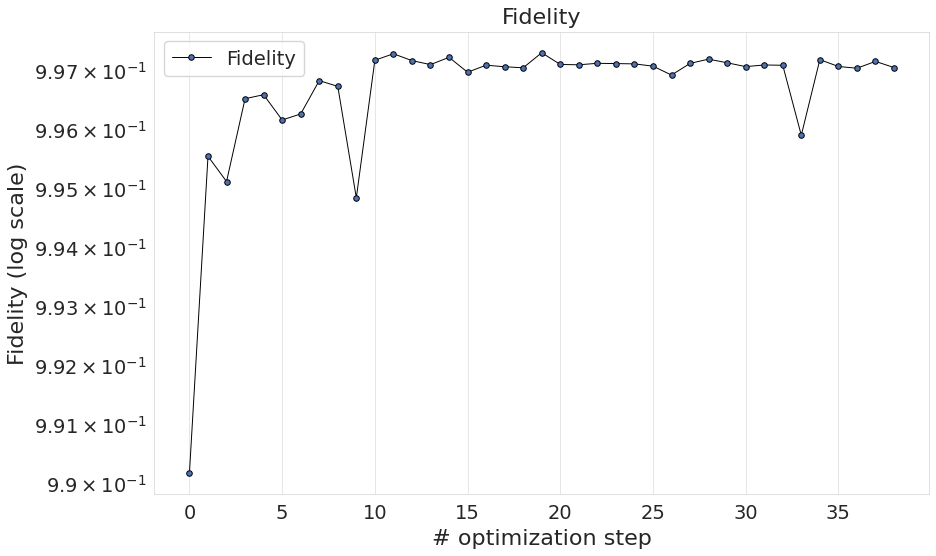
\includegraphics[width=\textwidth]{figures/png/RB_optimization/NM/post_ft_true/NM_fid.png}
        \caption{Plot of the average Clifford gate fidelity as a function of the function evaluations.}
        \label{NM_true_fig:fidelity}
    \end{subfigure}
    \hfill
    \begin{subfigure}[t]{0.45\textwidth}
        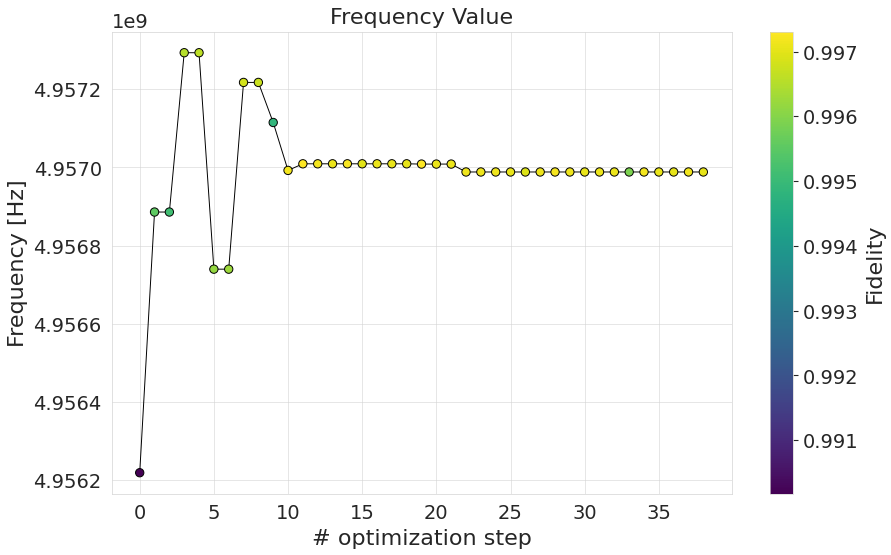
\includegraphics[width=\textwidth]{figures/png/RB_optimization/NM/post_ft_true/frequency.png}
        \caption{Plot of the frequency of the $R_X$ gate corresponding to different optimization steps.}
        \label{NM_true_fig:frequency}
    \end{subfigure}

    \vspace{0.5cm}

    \begin{subfigure}[t]{0.45\textwidth}
        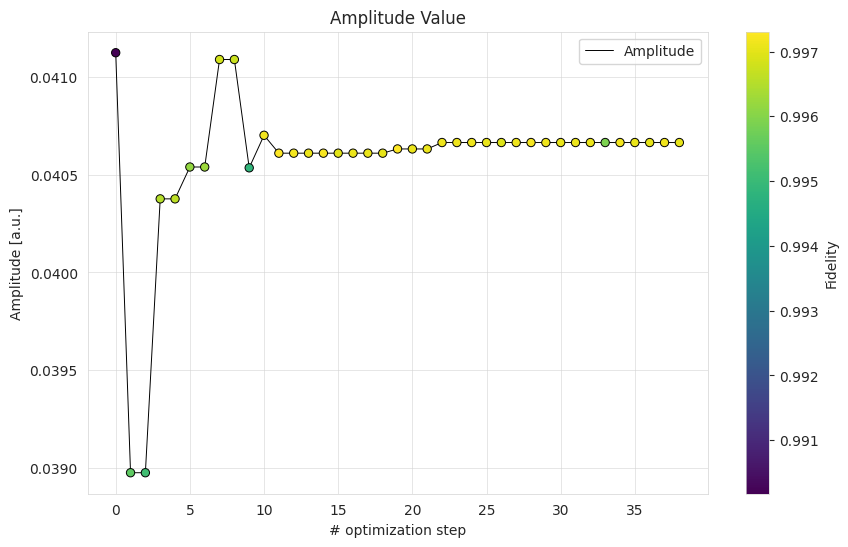
\includegraphics[width=\textwidth]{figures/png/RB_optimization/NM/post_ft_true/amplitude.png}
        \caption{Plot of the amplitude of the $R_X$ gate corresponding to different optimization steps.}
        \label{NM_true_fig:amplitude}
    \end{subfigure}
    \hfill
    \begin{subfigure}[t]{0.45\textwidth}
        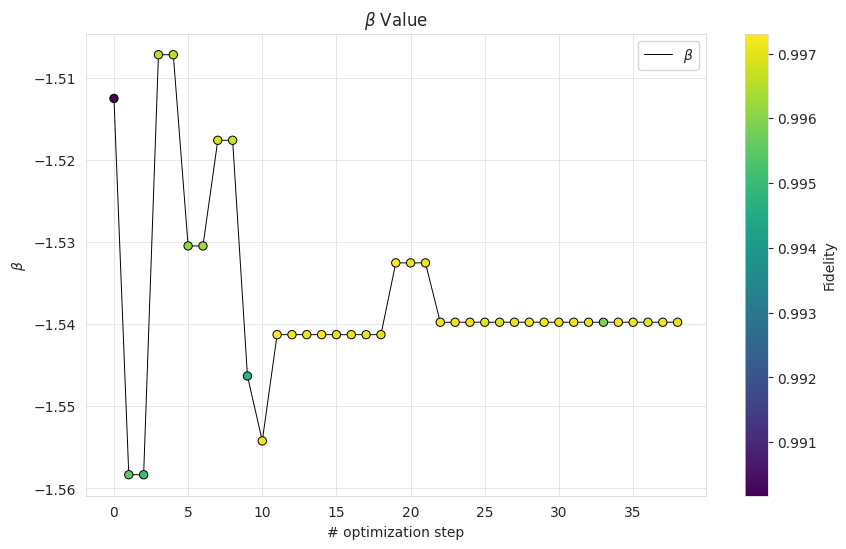
\includegraphics[width=\textwidth]{figures/png/RB_optimization/NM/post_ft_true/beta.png}
        \caption{Plot of the $\beta$ multiplying coefficient for the second quadrature component of the DRAG pulse.}
        \label{NM_true_fig:beta}
    \end{subfigure}

    \caption{Plots of the fidelity and optimization parameters as a function of the number of optimization step.}
    \label{fig:NM_plots}
\end{figure}

In Figure \ref{NM_true_fig:fidelity}, the evolution of the fidelity during the optimization is shown. 
The corresponding values of the parameters being optimized are reported in Figures \ref{NM_true_fig:frequency}, \ref{NM_true_fig:amplitude}, and \ref{NM_true_fig:beta}. 
From these plots, it is again evident that the optimization is converging (possibly to a local minimum) as the parameters stabilize around specific values: \texttt{amplitude} $= 0.04$, \texttt{frequency} $= 4.957$ GHz, and \texttt{beta} $= -1.54$.

However, a possible limitation to the performance of this optimization approach may lie in the absence of an explicitly defined initial simplex.
Setting only the initial parameter values, without specifying the full simplex, can lead the algorithm to explore the parameter space inefficiently. 
For this reason, further runs of the same method were carried out, this time also initializing the simplex explicitly.

Furthermore, considering that the allowed variation range for the $\beta$ parameter was restricted to only $\pm0.25$ around the value determined by the \tt{drag\_tuning} routine, I explored the possibility of improving the efficiency of the optimization by reducing the number of free parameters. 
Specifically, additional optimization runs were performed in which only the amplitude and frequency of the $R_X$ pulse were optimized, while $\beta$ was kept fixed.

This choice was motivated by the working assumption that, at least in this initial phase, leakage errors were not the dominant source of infidelity. 
Since the DRAG correction primarily addresses leakage to higher energy levels, it was hypothesized that optimizing $\beta$ would have a limited effect on the overall gate fidelity compared to the more significant impact of accurately calibrating the native gate's amplitude and frequency. 
As such, the focus was placed on parameters expected to yield the greatest improvements in fidelity while maintaining a limited run time.

Some optimization runs were performed with this nrevised configuration.
The results of these runs are reported in the following sections and are labeled as \tt{init\_symp\_1}, \tt{init\_symp\_2}, and \tt{init\_symp\_3}.

\begin{figure}
    \centering
    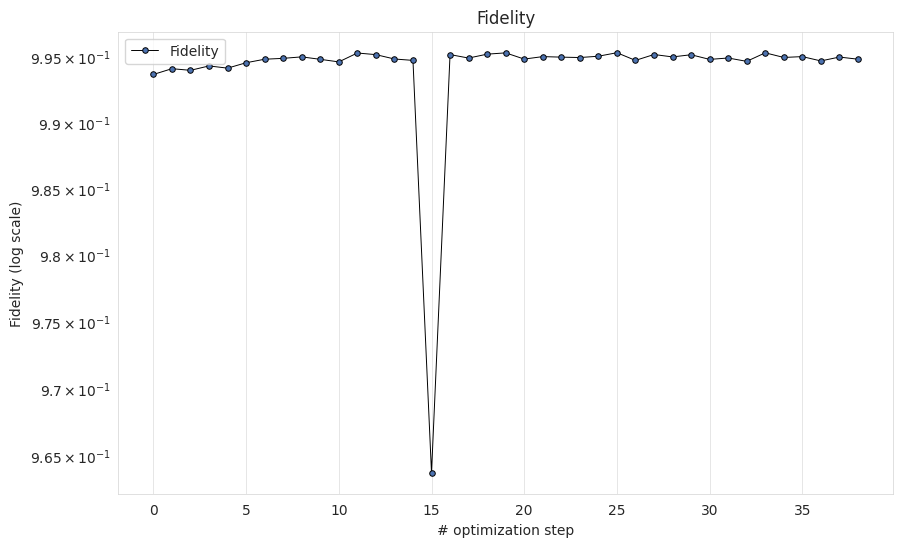
\includegraphics[width=0.45\textwidth]{figures/png/RB_optimization/NM/InitialSymplex/20241110_211211/fidelity.png}
    \caption{Plot of the average Clifford gate fidelity as a function of the optimization steps for the first round optimization - \tt{init\_symp\_1}.}
    \label{fig:20241110_211211:fidelity}
\end{figure}

\begin{figure}[htbp]
    \centering
    \begin{subfigure}[t]{0.45\textwidth}
        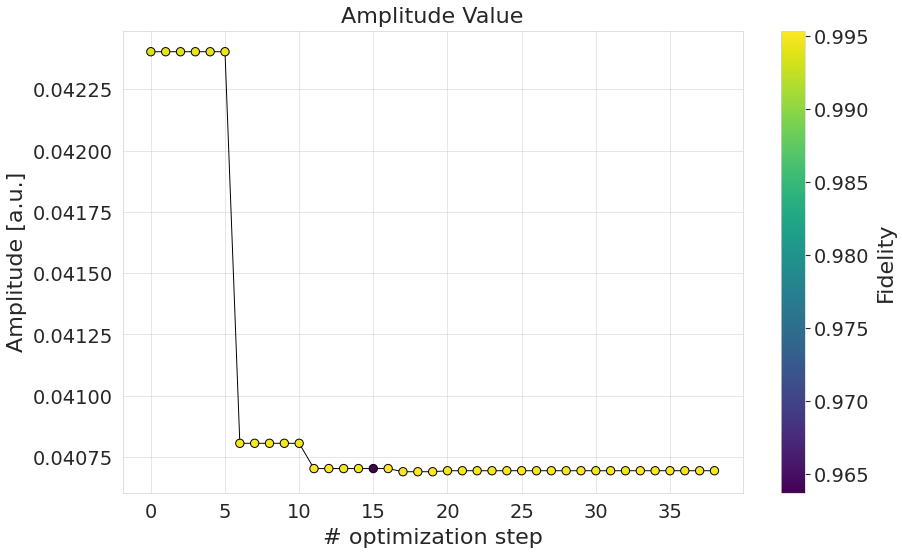
\includegraphics[width=\textwidth]{figures/png/RB_optimization/NM/InitialSymplex/20241110_211211/amplitude.png}
        \caption{Plot of the amplitude of the $R_X$ gate corresponding to different optimization steps.}
        \label{fig:20241110_211211:amplitude}
    \end{subfigure}
    \hfill
    \begin{subfigure}[t]{0.45\textwidth}
        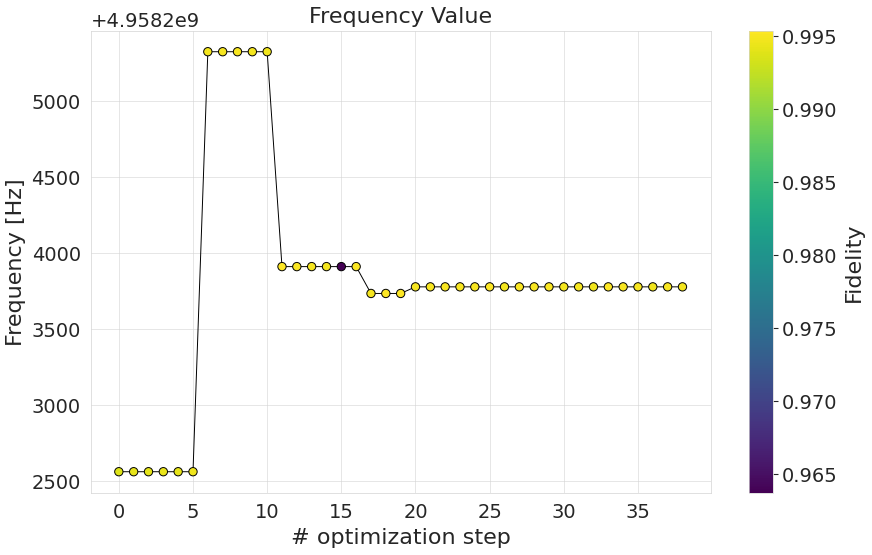
\includegraphics[width=\textwidth]{figures/png/RB_optimization/NM/InitialSymplex/20241110_211211/frequency.png}
        \caption{Plot of the frequency of the $R_X$ gate corresponding to different optimization steps.}
        \label{fig:20241110_211211:frequency}
    \end{subfigure}
    \caption{Plots of the optimization parameters as a function of the number of optimization step for the first round optimization - \tt{init\_symp\_2}.}
    \label{fig:20241110_211211:parameters}
\end{figure}

\begin{figure}
    \centering
    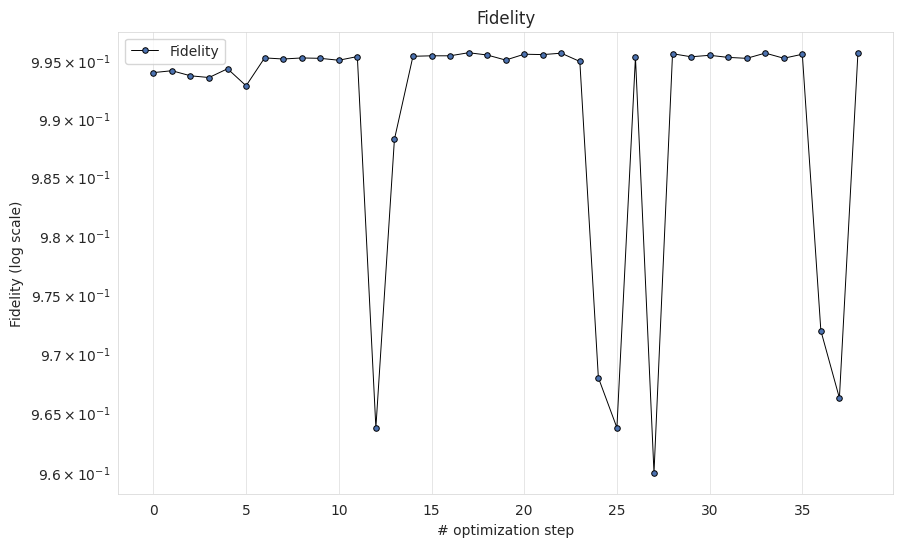
\includegraphics[width=0.45\textwidth]{figures/png/RB_optimization/NM/InitialSymplex/20241113_181711/fidelity.png}
    \caption{Plot of the average Clifford gate fidelity as a function of the optimization steps for the second round optimization - \tt{init\_symp\_2}.}
    \label{fig:20241113_181711:fidelity}
\end{figure}

\begin{figure}[htbp]
    \centering
    \begin{subfigure}[t]{0.45\textwidth}
        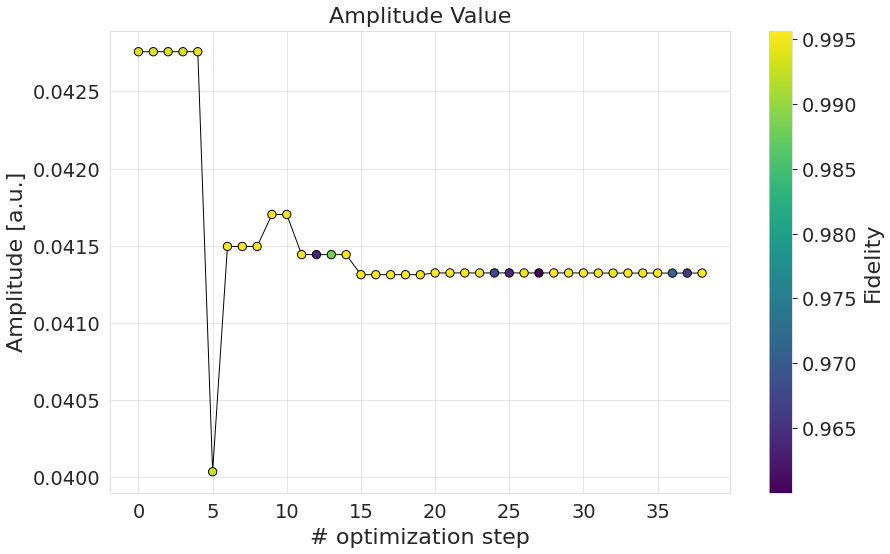
\includegraphics[width=\textwidth]{figures/png/RB_optimization/NM/InitialSymplex/20241113_181711/Amplitude.png}
        \caption{Plot of the amplitude of the $R_X$ gate corresponding to different optimization steps.}
        \label{fig:20241113_181711:amplitude}
    \end{subfigure}
    \hfill
    \begin{subfigure}[t]{0.45\textwidth}
        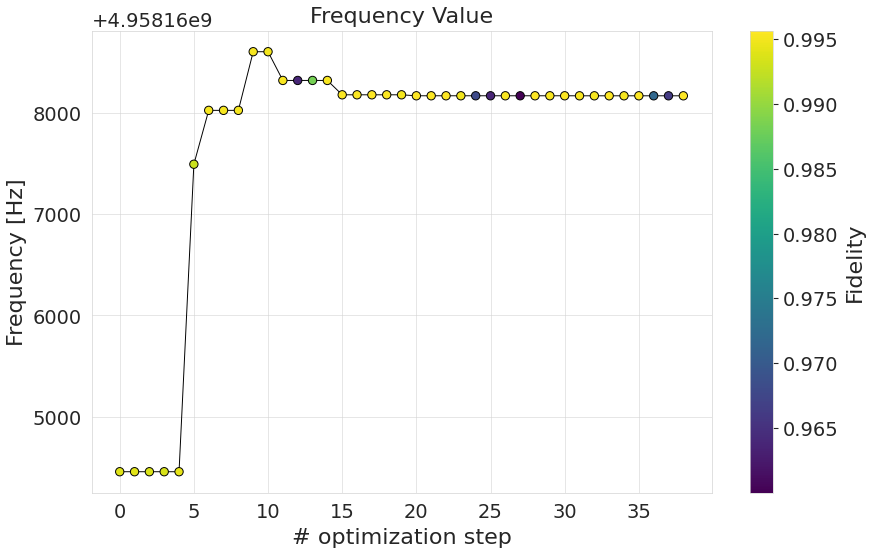
\includegraphics[width=\textwidth]{figures/png/RB_optimization/NM/InitialSymplex/20241113_181711/Frequency.png}
        \caption{Plot of the frequency of the $R_X$ gate corresponding to different optimization steps.}
        \label{fig:20241113_181711:frequency}
    \end{subfigure}
    \caption{Plots of the optimization parameters as a function of the number of optimization steps for the first round optimization - \tt{init\_symp\_2}.}
    \label{fig:20241113_181711:parameters}
\end{figure}

\begin{figure}
    \centering
    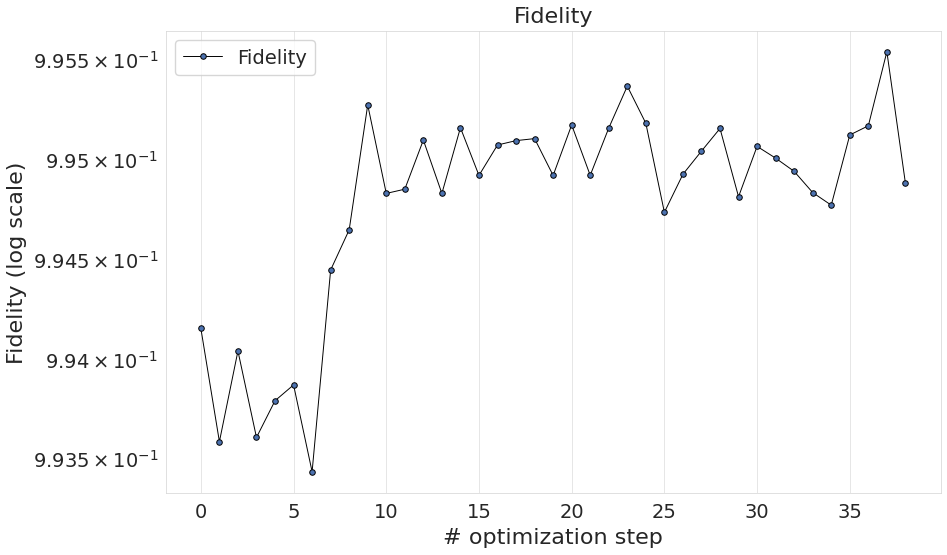
\includegraphics[width=0.45\textwidth]{figures/png/RB_optimization/NM/InitialSymplex/20241113_200745/fidelity.png}
    \caption{Plot of the average Clifford gate fidelity as a function of the optimization steps for the first round optimization - \tt{init\_symp\_3}.}
    \label{fig:20241113_200745:fidelity}
\end{figure}

\begin{figure}[htbp]
    \centering
    \begin{subfigure}[t]{0.45\textwidth}
        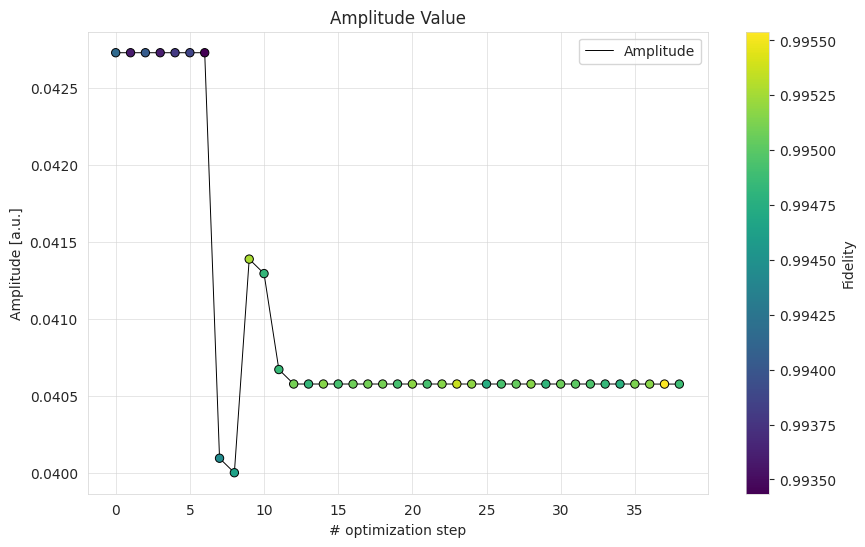
\includegraphics[width=\textwidth]{figures/png/RB_optimization/NM/InitialSymplex/20241113_200745/Amplitude.png}
        \caption{Plot of the amplitude of the $R_X$ gate corresponding to different optimization steps.}
        \label{fig:20241113_200745:amplitude}
    \end{subfigure}
    \hfill
    \begin{subfigure}[t]{0.45\textwidth}
        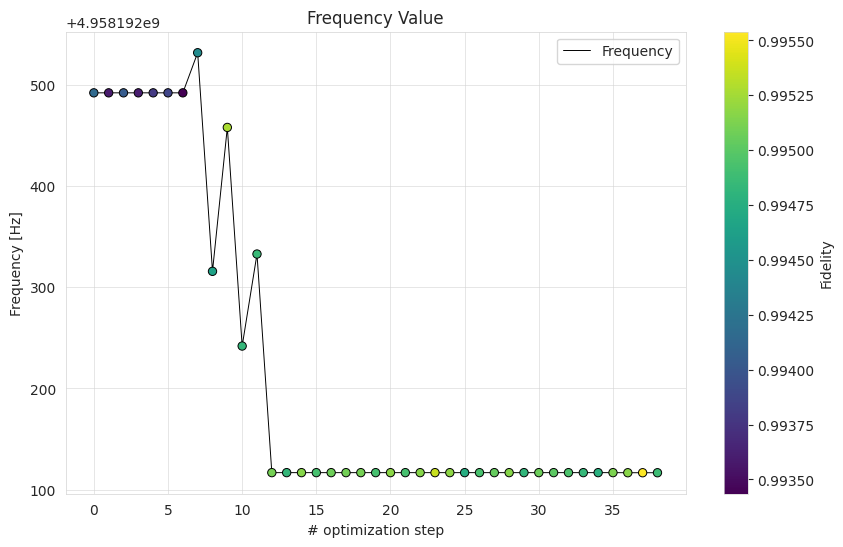
\includegraphics[width=\textwidth]{figures/png/RB_optimization/NM/InitialSymplex/20241113_200745/Frequency.png}
        \caption{Plot of the frequency of the $R_X$ gate corresponding to different optimization steps.}
        \label{fig:20241113_200745:frequency}
    \end{subfigure}
    \caption{Plots of the optimization parameters as a function of the number of optimization step for the first round optimization - \tt{init\_symp\_3}.}
    \label{fig:20241113_200745:parameters}
\end{figure}


Un riassunto dei risultati ottenuti utilizzando l'algoritmo di Nelder-Mead nelle diverse configurazioni è riportato nelle prime righe di Table \ref{tab:scipy_opt}.
    
\subsection{SLSQP}
\subsubsection{Algorithm description}
Per valutare eventuali miglioramenti nella performance abbiamo provato ad utilizzare un algoritmo che fosse gradient-based. 
Nello specifico ho provato ad utilizzare l'algoritmo di Sequential Least Squares Programming (SLSQP) nella versione implementata all'interno della libreria \tt{SciPy}.

The Sequential Least Squares Programming (SLSQP) method, originally developed by Dieter Kraft in 1988 \cite{kraft1988slsqp}, is a gradient-based algorithm for solving constrained nonlinear optimization problems.
The algorithm solves a nonlinear constrained problem of the form:
\begin{align*}
& \min_{x \in \mathbb{R}^n} \quad && f(x) \\
& \text{subject to} \quad && c_i(x) = 0, \quad i = 1, \dots, m \\
& && d_j(x) \geq 0, \quad j = 1, \dots, p
& && \mathbf{x}^{(L)} \leq \mathbf{x} \leq \mathbf{x}^{(U)}
\end{align*}

It belongs to the class of Sequential Quadratic Programming (SQP) methods, which iteratively solve a sequence of quadratic programming subproblems that locally approximate the original nonlinear problem. 
\begin{enumerate}
    \item \textit{Linearization}: At iteration $k$, the nonlinear constraints are approximated by their first-order Taylor expansion around the current point $\mathbf{x}_k$.
    This transforms the nonlinear constraints into a linear system locally.
    \item \textit{Quadratic subproblem construction}: The objective is approximated by a quadratic model of the Lagrangian function: \begin{equation}
        \mathcal{L}(\mathbf{x}, \lambda, \mu) = f(\mathbf{x}) - \sum_{i=1}^{m} \lambda_i c_i(\mathbf{x}) - \sum_{j=1}^{p} \mu_j d_j(\mathbf{x}),
    \end{equation}
    where $\lambda_i$ and $\mu_j$ are Lagrange multipliers. 
    The Hessian of the Lagrangian is not computed explicitly, but approximated using a BFGS-like quasi-Newton update.
    \item \textit{QP Subproblem solution}: A quadratic program is solved to determine a search direction $\mathbf{p}_k$, subject to the linearized constraints and bounds. 
    The subproblem minimizes the quadratic model subject to these constraints.
    \item \textit{Constrained line search}: A line search is performed along $\mathbf{p}_k$ using a merit function that balances reduction in the objective with feasibility of constraints. 
    This helps ensure global convergence.
    \item \textit{Update}: The iterate is updated via $\mathbf{x}_{k+1} = \mathbf{x}_k + \alpha_k \mathbf{p}_k$, where $\alpha_k$ is the step size determined by the line search. 
    The quasi-Newton approximation of the Hessian is also updated.
    \item \textit{Termination}: The algorithm terminates when the norm of the projected gradient and constraint violations fall below a specified tolerance.
\end{enumerate}

If analytic derivatives for the objective or constraints are not provided, they are approximated using forward finite differences. 
In such cases, each gradient estimation requires $n+1$ function evaluations per iteration, where $n$ is the number of variables.
The values of internal parameters, such as merit function balancing terms and quasi-Newton updates, are managed internally and are not user-configurable through \tt{SciPy}.

\subsubsection{Results}
\begin{figure}[htbp]
    \centering
    \begin{subfigure}[t]{0.45\textwidth}
        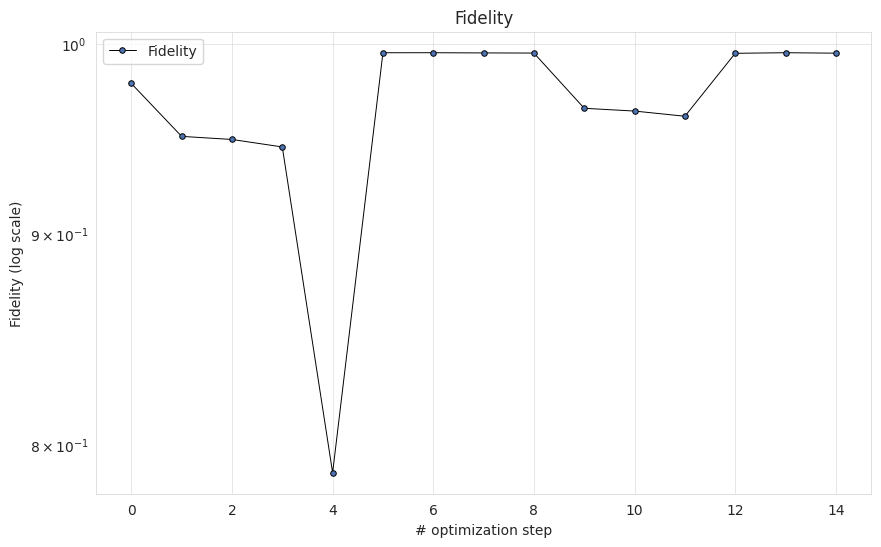
\includegraphics[width=\textwidth]{figures/png/RB_optimization/SLSQP/fidelity.png}
        \caption{Plot of the average Clifford gate fidelity as a function of the optimization steps.}
        \label{NM_true_fig:fidelity}
    \end{subfigure}
    \hfill
    \begin{subfigure}[t]{0.45\textwidth}
        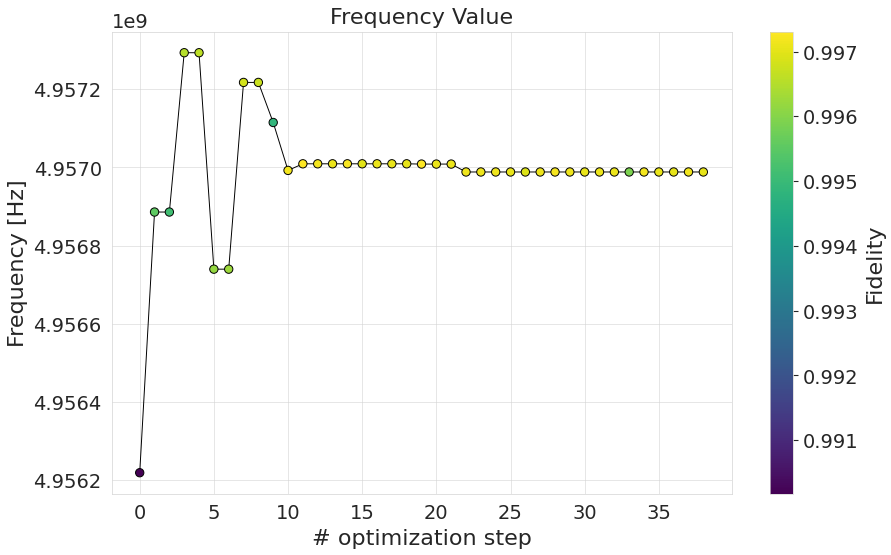
\includegraphics[width=\textwidth]{figures/png/RB_optimization/NM/post_ft_true/frequency.png}
        \caption{Plot of the frequency of the $R_X$ gate corresponding to different optimization steps.}
        \label{NM_true_fig:frequency}
    \end{subfigure}

    \vspace{0.5cm}

    \begin{subfigure}[t]{0.45\textwidth}
        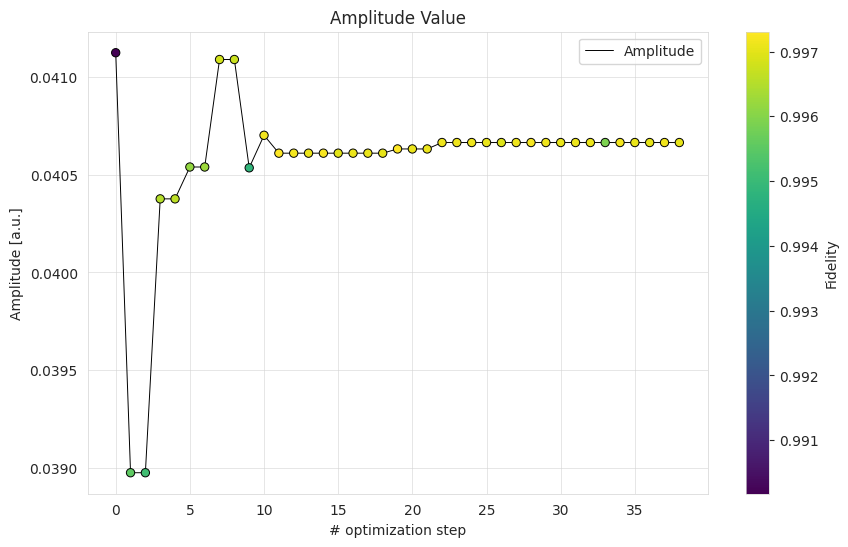
\includegraphics[width=\textwidth]{figures/png/RB_optimization/NM/post_ft_true/amplitude.png}
        \caption{Plot of the amplitude of the $R_X$ gate corresponding to different optimization steps.}
        \label{NM_true_fig:amplitude}
    \end{subfigure}
    \hfill
    \begin{subfigure}[t]{0.45\textwidth}
        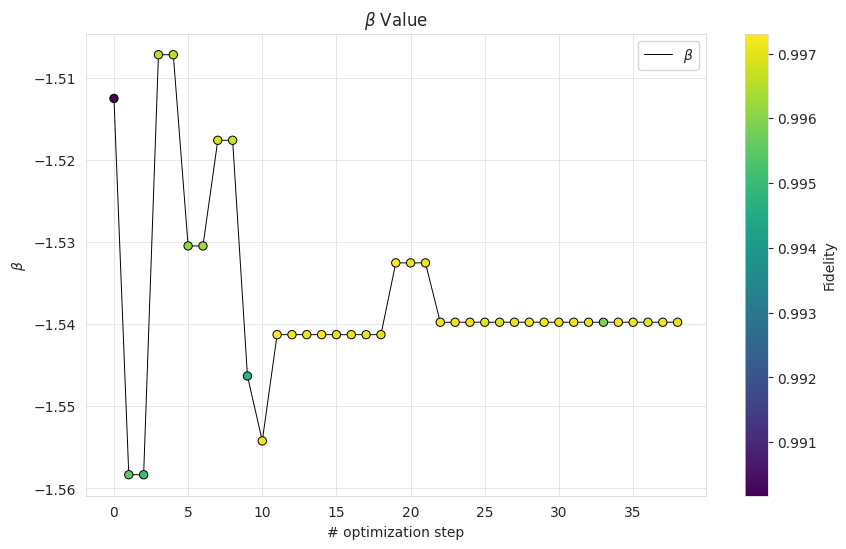
\includegraphics[width=\textwidth]{figures/png/RB_optimization/NM/post_ft_true/beta.png}
        \caption{Plot of the $\beta$ multiplying coefficient for the second quadrature component of the DRAG pulse.}
        \label{NM_true_fig:beta}
    \end{subfigure}

    \caption{Plots of the fidelity and optimization parameters as a function of the number of optimization step for the SLSQP optimization method.}
    \label{fig:NM_plots}
\end{figure}

\begin{table}[h]
    \centering
    \begin{tabular}{lcccccc}
        \toprule
        \textbf{Method} & \textbf{Success} & \textbf{Objective Value} & \textbf{Iterations} & \textbf{Function Evaluations} & \textbf{Duration [s]}\\
        \hline
        \textbf{Nelder-Mead} & False & 0.002732 & 40 & 93 & 2892 \\
        \textbf{init\_symplex\_1} & False & & 40 & 99 & 3096\\
        \textbf{init\_symplex\_2} & False & & 40 & 100 & 3128\\
        \textbf{init\_symplex\_3} & False & & 40 & 106 & 3190\\
        \textbf{SLSQP} & True & & 15 & 180 & 3873\\
        \bottomrule
    \end{tabular}
    \caption{}
    \label{tab:scipy_opt}
\end{table}


\section{CMA-ES}

\subsection{Algorithm description}
Covariance Matrix Adaptation Evolution Strategy (\tt{CMA-ES} \cite{cmaessimplepractical}), is a population-based evolutionary algorithm designed for optimizing complex, non-convex, and high-dimensional functions.\\
It belongs to the broader class of Evolution Strategies (ES), a subset of Evolutionary Algorithms (EAs)(see \cite{sloss20192019evolutionaryalgorithmsreview}), and is particularly effective for black-box optimization where gradient information is unavailable.

Evolution Strategies (ES) are a class of optimization methods that employ self-adaptive mechanisms to explore the search space efficiently. 
Unlike classical optimization techniques that rely on gradient descent, ES leverage stochastic sampling to navigate rugged and multimodal landscapes.
In this context, CMA-ES is an adaptive stochastic search method that iteratively refines a probability distribution over the search space. 
Unlike traditional Genetic Algorithms (GAs), which rely on crossover and mutation operators, CMA-ES employs a multivariate normal distribution to generate candidate solutions. 
The method adaptively updates the distribution's mean and covariance matrix based on the fitness of sampled points.

The fundamental idea behind CMA-ES is the use of a multivariate Gaussian distribution to model promising search directions. 
Let $\mathbf{\mu}_t$ denote the mean of the distribution at iteration $t$, and $\Sigma_t$ the covariance matrix. 
Then, a new population of $\lambda$ candidate solutions $\mathbf{x}_i^{(t+1)} \sim \mathbf{\mu}_t + \sigma_t\mathcal{N}(0, \Sigma_t)$, where $\sigma_t$ is a step size controlling the exploration.  

The CMA-ES algorithm follows the following steps:\begin{enumerate}
    \item If not otherwise specified, the initial parameters are set: mean vector $\mathbf{\mu_0}$, covariance matrix $\Sigma_0$\footnote{$\Sigma_0=\mathbb{I}$ for isotropic search}, step size $\sigma_0$, population size $\lambda$
    \item Generate $\lambda$ new candidate solutions $\mathbf{x}_i$ according to a multivariate normal distribution.
    \item Evaluate the objective function $f(\mathbf{x}_i)$ for each candidate solution.
    \item Sort the new candidate solutions based on fitness: $f(\mathbf{x}_0) \leq ... \leq f(\mathbf{x}_{\lambda})$.
    \item Update the mean vector $\mathbf{\mu}$ with the $m=\lfloor \lambda / 2 \rfloor$ top performing solutions:\begin{equation}
        \mathbf{\mu} \leftarrow \sum_{i=0}^m \mathbf{w}_i\mathbf{x}_1,
    \end{equation} where $\mathbf{w}_i$ are internally defined weights.
    \item Update the isotropic and anisotropic evolution path $\mathbf{p}_{\sigma}$, $\mathbf{p}_c$ \footnote{For details on the update process of the evolution paths see \cite{cmaessimplepractical}.}.
    \item Update the covariance matrix: \begin{equation}
        C \leftarrow (1 - c_1 - c_{\mu}) C + c_1 \mathbf{p}_c \mathbf{p}_c^T + c_{\mu} \sum_{i=1}^{\mu} w_i \mathbf{y}_i \mathbf{y}_i^T,
    \end{equation} where $c_1$ and $c_\mu$ are learning rates and $\mathbf{y}_i$ represents the deviation of the $i$-th cnadidate solution from the mean $\mathbf{mu}$.
    \item Update the step size using a cumulative path evolution mechanism \begin{equation}
        \sigma \leftarrow \sigma \cdot \exp \left( \frac{c_{\sigma}}{d_{\sigma}} \left( \| \mathbf{p}_{\sigma} \| - E \| \mathcal{N}(0, I) \| \right) \right),
    \end{equation} where $c_\sigma$ is the learning rate for step-size adaptation, $d_\sigma$ is a damping factor $\| \mathbf{p}_{\sigma} \|$ is the length of the evolution path and $E \| \mathcal{N}(0, I) \|$ is the expected length of a standard normally distributed random vector.
\end{enumerate}

Nel seguito, a meno che non sia diversamente specificato, i parametri sono stati inizializzati ai valori di default della libereria \tt{CMA-ES}
\subsection{Results}


\section{Optuna}

\subsection{Algorithm description}

In addition to the optimization methods mentioned earlier, the Tree-Structured Parzen Estimator (TPE) method was employed, using its implementation available in the \texttt{optuna} library \cite{optuna_2019}.

Tree-Structured Parzen Estimator (TPE) is a Sequential Model-Based Optimization (SMBO) approach \cite{SMBO_proceedings}. 
SMBO methods sequentially construct models to approximate the performance of optimization parameters based on historical measurements, and then subsequently choose new parameters values to test based on this model. \cite{BayesianOptimizationReview}
At the heart of SMBO is the idea of building a surrogate model, which is used to predict the objective function's values for unseen parameters configurations. 
The surrogate model is iteratively updated as new observations are made, and the optimization process balances exploration, which focuses on uncertain regions of the search space, and exploitation, which focuses on areas that are more likely to improve the objective based on past evaluations. 
This balance ensures that the optimization process makes efficient use of resources and avoids wasting time on suboptimal regions.\\

The TPE algorithm is a probabilistic model-based optimization method that uses non-parametric density estimation to guide the search. 
The TPE algorithm differs from traditional Bayesian optimization approaches, such as Gaussian Process-based methods, in its modeling strategy. 
Rather than directly approximating the objective function, TPE constructs two separate probabilistic models:

\begin{itemize}
    \item $p(x | y < y^*)$, the likelihood of observing a parameter configuration $x$ given that the objective function value $y$ is below a chosen threshold $y^*$.
    \item $p(x | y \geq y^*)$, the likelihood of observing $X$ for less promising function values.
\end{itemize}

These probability densities are estimated using non-parametric methods such as kernel density estimation (KDE). 
New candidate points are then generated by sampling from $p(x | y < y^*)$, favoring configurations that are expected to yield lower objective values. The threshold $y^*$ is typically set as a quantile of observed values, ensuring a focus on the most promising regions of the search space.

The TPE method is the default optimization strategy in \tt{Optuna}, an advantage in the optimization algorithm as implemented in optuna is the addition of an authomatic \textit{pruning} mechanism that stops  unpromising trials early, which can significantly speed up the optimization process by avoiding unnecessary computations.
In our case, this is particularly relevant because the execution of the RB routine, which is performed at each call to the cost function, requires [insert approximate execution time]

As implemented in our code, the default pruner used is the median pruner \tt{optuna.pruners.MedianPruner}. 
This pruner works by evaluating the intermediate results of a trial and comparing them to the median of completed trials at the same step. 
If the current trial's performance is worse than the median, it is pruned to prevent wasting computational resources on unpromising configurations. 

\subsection{Results}

\subsection{$\beta$ parameter impact on RB optimization}

\paragraph{D1 - steps}

\paragraph{D1 - 1000 steps}

\paragraph{D2 - 1000 steps}



\section{RB optimization conclusions}
As mentioned in the introduction to this chapter, the primary objective of this work was to evaluate whether it is possible to develop an automated optimization routine that can be executed directly on quantum hardware to periodically improve the fidelity of single-qubit gates—specifically the  $R_X(\pi)$ gate. 
For such a routine to be practically useful, two main conditions must be met: first, the optimization must lead to a consistent and measurable improvement in gate fidelity within a limited amount of time; 
second, the routine must demonstrate stable convergence, such that the resulting optimized parameters (amplitude, frequency, and DRAG correction) can reliably be used to update the hardware configuration, ensuring a reproducible improvement in performance.

While the protocol did yield fidelity improvements in several cases, the results indicate that the implementation we built to be run on hardware is not yet robust or efficient enough for routine use. 
The main limiting factor is the duration of the Randomized Benchmarking routine used to evaluate gate fidelity, which is relatively long. 
Because the optimization procedure requires several evaluations of this cost function, the total execution time quickly becomes a bottleneck. 
Furthermore, we observed that convergence is not always guaranteed: in some cases, the optimization either stalls or does not lead to meaningful improvements within the time frame or number of iterations considered acceptable for practical deployment.

In summary, although the method shows that automated gate fidelity optimization is possible, the current implementation does not meet the reliability and efficiency requirements needed for scheduled, hardware-level recalibration. 
Improvements could focus on accelerating cost function evaluation or designing more robust optimization strategies with stronger convergence guarantees.

\begin{comment}
\begin{tabular}{lccccc}
    \textbf{Method} & \textbf{Highest Fidelity} & \textbf{Amplitude [a.u.]} & \textbf{Frequency [GHz]} & \textbf{$\beta$} \\

\end{tabular}

\begin{tabular}{lcccccccccccccccccc}
\textbf{Analysis Name} & \textbf{cost\_initial} & \textbf{cost\_best} & \textbf{index\_best} & \textbf{A best [a.u.]} & \textbf{f best [$\times10^9$ Hz]} & \textbf{B best} & \textbf{cost\_final} & \textbf{A final [a.u.]} & \textbf{f final [$\times10^9$ Hz]} & \textbf{B final} & \textbf{improv. best [\%]} & \textbf{improv. final [\%]} & \textbf{fid\_initial} & \textbf{fid\_best} & \textbf{fid\_final} & \textbf{fid impr. best [\%]} & \textbf{fid impr. final [\%]} \\
\hline
D1\_cma\_post\_ft\_true & 0.00728 & 0.00335 & 9 & -0.16634 & 4.95822 & 0.08802 & 0.02664 & 0.12956 & 4.95822 & 0.18364 & 54.04 & -265.93 & 0.99272 & 0.99665 & 0.97336 & 0.40 & -1.95 \\
D1\_init\_simplex\_20241110\_211211 & 0.00633 & 0.00467 & 25 & 0.04069 & 4.95820 &  & 0.00517 & 0.04069 & 4.95820 &  & 26.23 & 18.41 & 0.99367 & 0.99533 & 0.99483 & 0.17 & 0.12 \\
D1\_nelder-mead\_post\_ft\_true & 0.00983 & 0.00269 & 19 & 0.04063 & 4.95701 & -1.53253 & 0.00295 & 0.04067 & 4.95699 & -1.53976 & 72.59 & 70.02 & 0.99017 & 0.99731 & 0.99705 & 0.72 & 0.69 \\
D1\_init\_simplex\_20241113\_181711 & 0.00607 & 0.00436 & 17 & 0.04131 & 4.95817 &  & 0.00437 & 0.04132 & 4.95817 &  & 28.27 & 28.10 & 0.99393 & 0.99564 & 0.99563 & 0.17 & 0.17 \\
D1\_init\_simplex\_20241113\_200745 & 0.00585 & 0.00446 & 37 & 0.04058 & 4.95819 &  & 0.00512 & 0.04058 & 4.95819 &  & 23.73 & 12.46 & 0.99415 & 0.99554 & 0.99488 & 0.14 & 0.07 \\
D1\_SLSQP\_post\_ft\_true & 0.02172 & 0.00482 & 13 & 0.04058 & 4.95822 & -0.00115 & 0.00507 & 0.04058 & 4.95822 & -0.00115 & 77.79 & 76.64 & 0.97828 & 0.99518 & 0.99493 & 1.73 & 1.70 \\
\end{tabular}

\begin{table}[h]
    \centering
    \begin{tabular}{lccc}
        \textbf{Analysis Name} & \textbf{# function evaluations} & \textbf{# optimization steps} & \textbf{time [s]}
        \hline
        \textbf{D1\_nelder-mead\_post\_ft\_true} & 93 & 39 & 2892 \\
        \textbf{D1_SLSQP} & 180 & 15 & 3873 \\
        \textbf{D1\_cma\_post\_ft\_true} & 210 & 30 & 4836 \\
        \textbf{D1\_init\_simplex\_20241110\_211211} & 99 & 39 & 3096 \\
        \textbf{D1\_init\_simplex\_20241113\_181711} & 100 & 39 & 3128 \\
        \textbf{D1\_init\_simplex\_20241113\_200745} & 106 & 39 & 3190 \\
        \textbf{}
    \bottomrule
    \end{tabular}
    \caption{}
    \label{tab:cal_results}
\end{table}
\end{comment}